\documentclass[aspectratio=169]{beamer}

\usetheme{SimpleDarkBlue} % simple, clean theme
\usecolortheme{default}

\usepackage{graphicx}

\title[Multimodal Alignment in ChatGPT \& Gemini]{Evaluating Multimodal Alignment in ChatGPT and Gemini:\\
An Empirical Study of Inter- and Intra-Model Consistency}
\author[S. Napolitano]{Saverio Napolitano}
\institute[Mid Sweden University]{Mid Sweden University}
\date{\today}

\begin{document}

% ----------------------------------------------------------
\begin{frame}
  \titlepage
\end{frame}

% ----------------------------------------------------------
\begin{frame}{Overview}
  \tableofcontents
\end{frame}

% ----------------------------------------------------------
\section{Introduction and Problem}

\begin{frame}{Motivation}
  \begin{itemize}
    \item Text-to-image systems (e.g., ChatGPT+DALL--E, Gemini) are often
          evaluated with \textbf{automatic metrics}.
    \item Deployment decisions, however, rely on \textbf{human perception}
          and preferences:
      \begin{itemize}
        \item Which image variant would a user actually pick?
        \item How consistent are models when switching captions or generators?
      \end{itemize}
    \item Common perceptual/semantic metrics:
      \begin{itemize}
        \item LPIPS (deep feature distance),
        \item MS-SSIM (structural similarity),
        \item CLIP-based similarity.
      \end{itemize}
    \item \textbf{Core issue:} It is unclear how well these metrics track
          human preferences in realistic small-choice settings.
  \end{itemize}
\end{frame}

% ----------------------------------------------------------
\begin{frame}{Research Questions}
  \begin{block}{RQ1}
    How consistent, with respect to human preferences, are ChatGPT and Gemini
    in aligning descriptions and generations, both within the same
    model and across different models?
  \end{block}
  \vspace{2mm}
  \begin{block}{RQ2}
    How well do LPIPS, MS-SSIM, and CLIP-based similarity align with human judgments in this setting?
  \end{block}
  \vspace{2mm}
  \begin{itemize}
    \item Small, controlled study: 15 images, 4 variants each,
          10 human raters ranking the variants.
  \end{itemize}
\end{frame}

% ----------------------------------------------------------
\section{Method and Approach}

\begin{frame}{Image Variants and Setup}
  \begin{itemize}
    \item Dataset:
      \begin{itemize}
        \item 15 reference images, manually collected.
        \item Diverse content: people, objects, embedded text, nature, drawings.
      \end{itemize}
    \item For each reference:
      \begin{itemize}
        \item 4 generated variants (a)--(d).
        \item Each variant combines:
      %\end{itemize}
      \begin{itemize}
        \item Generator: Gemini vs ChatGPT/DALL--E.
        \item Caption source: Gemini vs ChatGPT.
      \end{itemize}
      \end{itemize}
    \item Mapping (Table I in paper):
      \begin{itemize}
        \item (a) Gemini generator + Gemini caption.
        \item (b) Gemini generator + ChatGPT caption.
        \item (c) ChatGPT generator + Gemini caption.
        \item (d) ChatGPT generator + ChatGPT caption.
      \end{itemize}
  %\end{itemize}
\end{itemize}
\end{frame}

% ----------------------------------------------------------
\begin{frame}{Reference Image 07}
  \begin{center}
    \rotatebox{180}{\includegraphics[width=0.7\textwidth,height=0.7\textheight,keepaspectratio]{../03_project/01_basic/data/07/07_ref.jpeg}}
  \end{center}
\end{frame}

% ----------------------------------------------------------
\begin{frame}{Image 07 Variants}
  \begin{center}
    \setlength{\tabcolsep}{2pt}
    \begin{tabular}{cc}
      \includegraphics[width=0.46\textwidth,height=0.36\textheight,keepaspectratio]{../03_project/01_basic/data/07/07_a.jpg} &
      \includegraphics[width=0.46\textwidth,height=0.36\textheight,keepaspectratio]{../03_project/01_basic/data/07/07_b.png} \\
      \scriptsize (a) & \scriptsize (b) \\
      \includegraphics[width=0.46\textwidth,height=0.36\textheight,keepaspectratio]{../03_project/01_basic/data/07/07_c.png} &
      \includegraphics[width=0.46\textwidth,height=0.36\textheight,keepaspectratio]{../03_project/01_basic/data/07/07_d.png}
      \\
      \scriptsize (c) & \scriptsize (d)
    \end{tabular}
  \end{center}
\end{frame}

% ----------------------------------------------------------
\begin{frame}{Human Evaluation}
  \begin{itemize}
    \item 10 student raters (balanced male/female).
    \item Online survey on laptop screens.
    \item For each image:
      \begin{itemize}
        \item All four variants shown side-by-side, along with the reference image.
        \item Raters give a \textbf{strict ranking} 1--4.
        \item Instructions: prioritize \textbf{semantic fidelity}
              to the reference image.
      \end{itemize}
    \item Inter-rater agreement per image via Kendall's \( W \),
          averaged to \( \bar{W} = 0.40 \) (moderate agreement).
    \item No personal or identifying data collected; raters were
          blind to model identities.
  \end{itemize}
\end{frame}

% ----------------------------------------------------------
\begin{frame}{Automatic Metrics and Evaluation Protocol}
  \begin{itemize}
    \item Three off-the-shelf metrics:
      \begin{itemize}
        \item LPIPS (AlexNet backbone) -- lower is better.
        \item MS-SSIM -- higher is better.
        \item CLIP cosine similarity (ViT-B/32) -- higher is better.
      \end{itemize}
    \item Preprocessing:
      \begin{itemize}
        \item Variants resized to match the reference image
              for perceptual metrics.
      \end{itemize}
    \item Evaluation protocol:
      \begin{itemize}
        \item Compute metric scores per image and variant.
        \item Convert scores to \textbf{ranks} per image.
        \item For each image: compute correlation (Kendall, Spearman,
              Pearson) between human mean ranks and metric ranks.
        \item Bootstrap CIs and Wilcoxon signed-rank tests on the
              15 per-image Spearman coefficients.
      \end{itemize}
  \end{itemize}
\end{frame}

% ----------------------------------------------------------
\section{Results}

\begin{frame}{Human Preferences (RQ1)}
  \begin{columns}[T]
    \begin{column}{0.52\textwidth}
      \small
      \begin{itemize}
        \item Top-1 rates over all images and raters:
          \begin{itemize}
            \item (a) Gemini+Gemini: \textbf{44\%}
            \item (b) Gemini+ChatGPT: 22\%
            \item (c) ChatGPT+Gemini: 13.3\%
            \item (d) ChatGPT+ChatGPT: 20.7\%
          \end{itemize}
        \item Average inter-rater agreement:
          \begin{itemize}
            \item \( \bar{W} = 0.40 \): moderate agreement.
          \end{itemize}
        \item \textbf{Interpretation}:
          \begin{itemize}
            \item There is a preferred variant, but human noise is non-negligible.
          \end{itemize}
      \end{itemize}
    \end{column}
    \begin{column}{0.45\textwidth}
      \begin{center}
        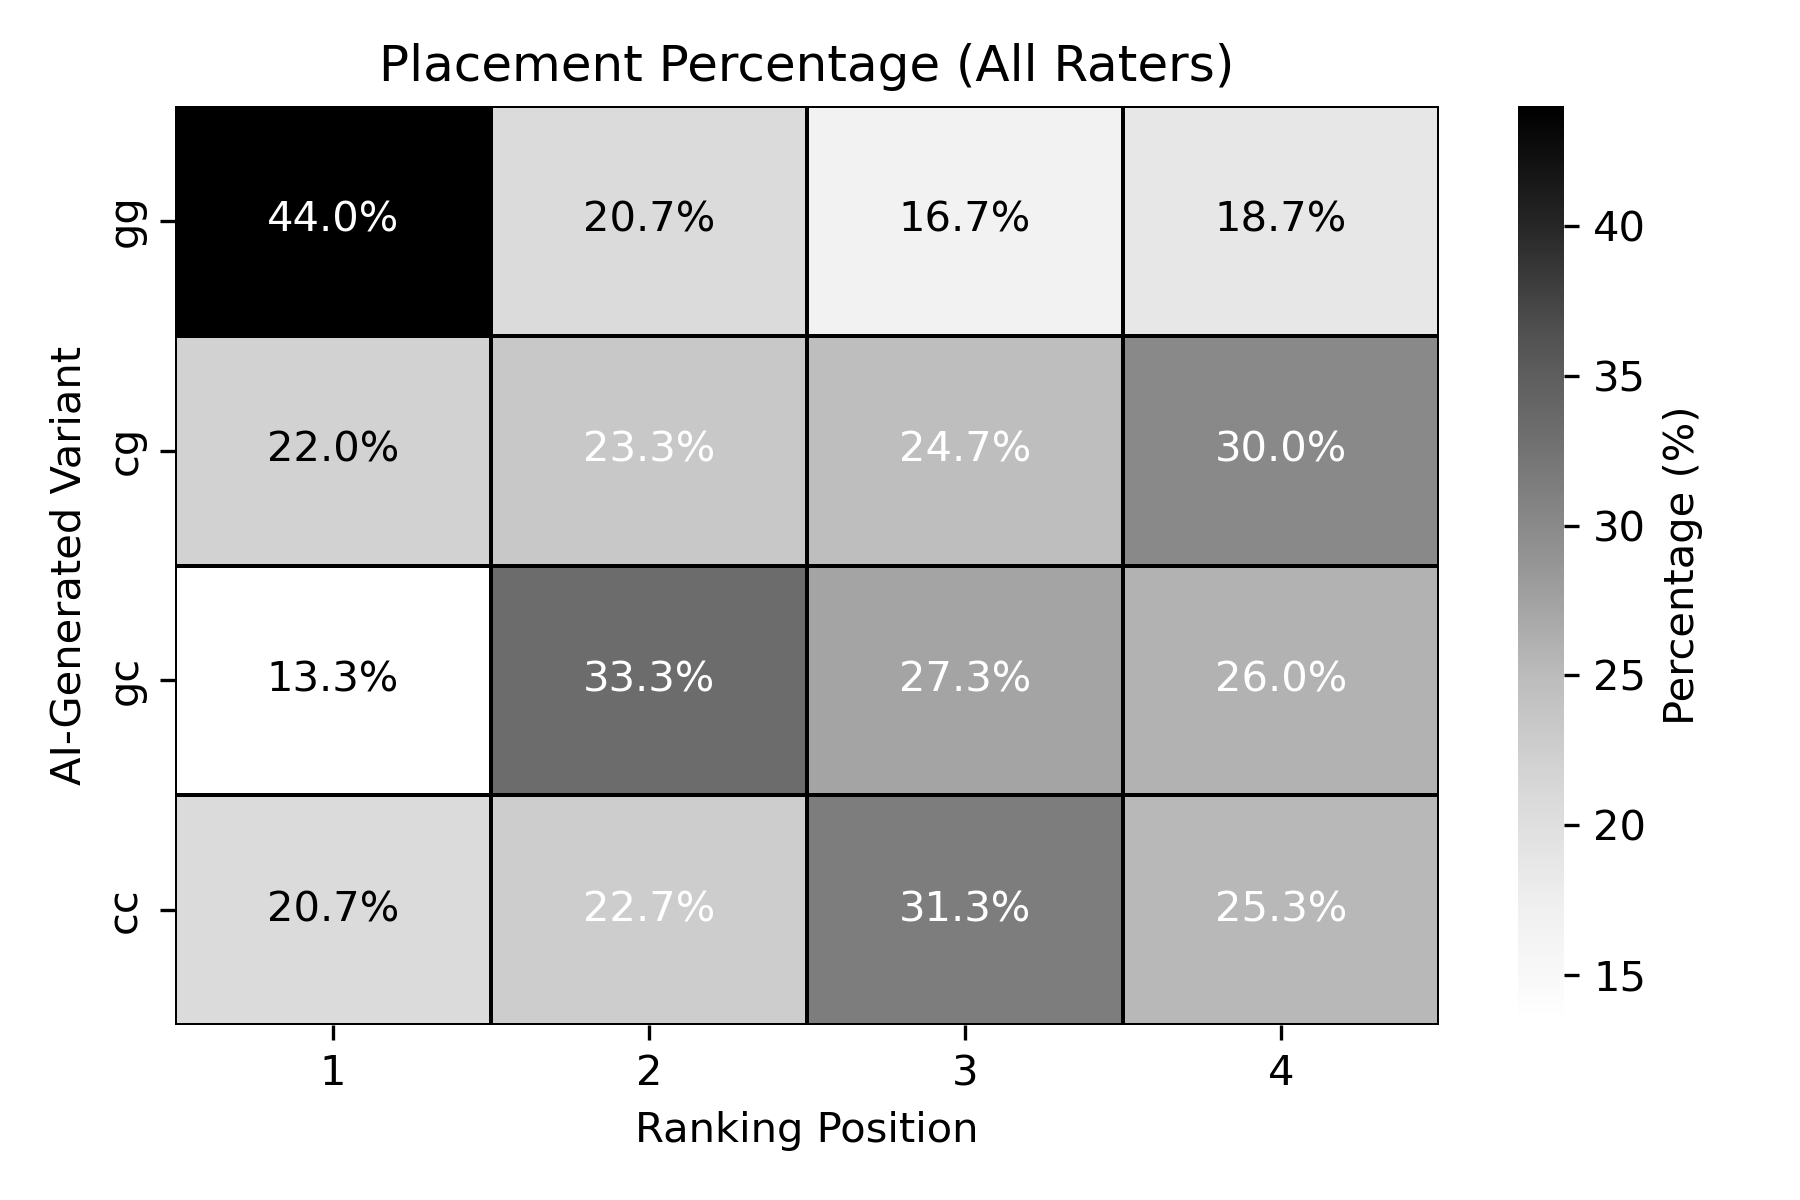
\includegraphics[width=\textwidth]{../03_project/01_basic/analysis/human_preferences_report/overall.png}
      \end{center}
      \vspace{-2mm}
      %\scriptsize Human placement percentages across variants.
    \end{column}
  \end{columns}
\end{frame}

% ----------------------------------------------------------
\begin{frame}{Inter- vs Intra-Model Consistency (RQ1)}
  \small

  % --- Top: text in two columns ---
  \begin{columns}[T,totalwidth=\textwidth]
    \begin{column}{0.48\textwidth}
      \begin{itemize}
        \item Pairs within each model:
          \begin{itemize}
            \item (a) vs (b): Gemini images, Gemini vs ChatGPT captions.
            \item (c) vs (d): ChatGPT images, Gemini vs ChatGPT captions.
          \end{itemize}
        \item Shares of comparisons:
          \begin{itemize}
            \item (a) $>$ (b): \textbf{62.7\%} vs 37.3\%.
            \item (c) $>$ (d): 47.3\% vs 52.7\%.
          \end{itemize}
      \end{itemize}
    \end{column}

    \begin{column}{0.48\textwidth}
      \begin{itemize}
        \item Mean rank differences:
          \begin{itemize}
            \item (a)--(b): mean \(-0.53\) ranks ((a) clearly better).
            \item (c)--(d): mean \(0.05\) (almost no difference).
          \end{itemize}
        \item \textbf{Interpretation:}
          \begin{itemize}
            \item ChatGPT is less sensitive to caption source
                  than Gemini in this setup.
          \end{itemize}
      \end{itemize}
    \end{column}
  \end{columns}

  \vfill

  % --- Bottom: full-width image ---
  \begin{center}
    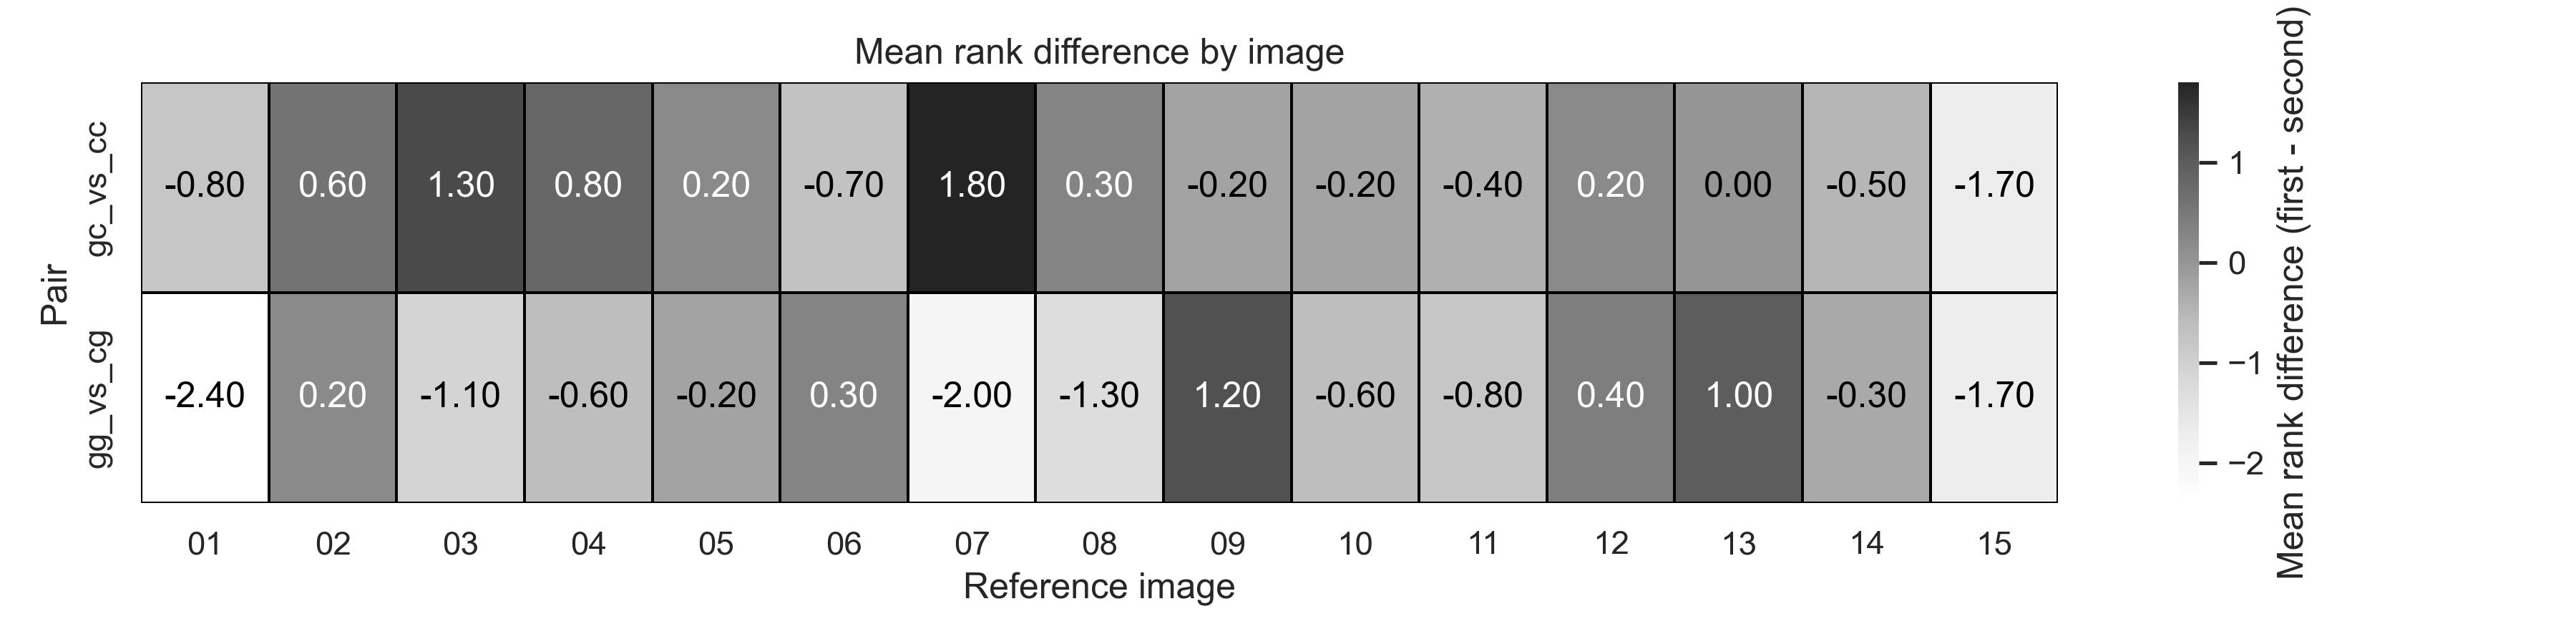
\includegraphics[width=0.8\textwidth]{../03_project/01_basic/analysis/pair_consistency_report/mean_rank_difference_heatmap.png}
  \end{center}
  \vspace{-2mm}
  %\scriptsize Mean rank difference per image for (a,b) and (c,d).
\end{frame}

% ----------------------------------------------------------
\begin{frame}{Metric Outcomes (RQ2) – Winners}
  \begin{columns}[T]
    \begin{column}{0.52\textwidth}
      \small
      \begin{itemize}
        \item Mean metric scores per variant (Table IV):
          \begin{itemize}
            \item All scores lie in a fairly narrow range.
            \item Metrics see variants as roughly similar in magnitude.
          \end{itemize}
        \item Global per-image wins:
          \begin{itemize}
            \item LPIPS: favors (a) most often (11.7\%).
            \item CLIP: favors (a) (10.0\%) and (d) (8.3\%).
            \item MS-SSIM: distributes wins across (b)--(d).
          \end{itemize}
        \item Indicates that metrics disagree with each other on
              which variant is “best”.
      \end{itemize}
    \end{column}
    \begin{column}{0.45\textwidth}
      \begin{center}
        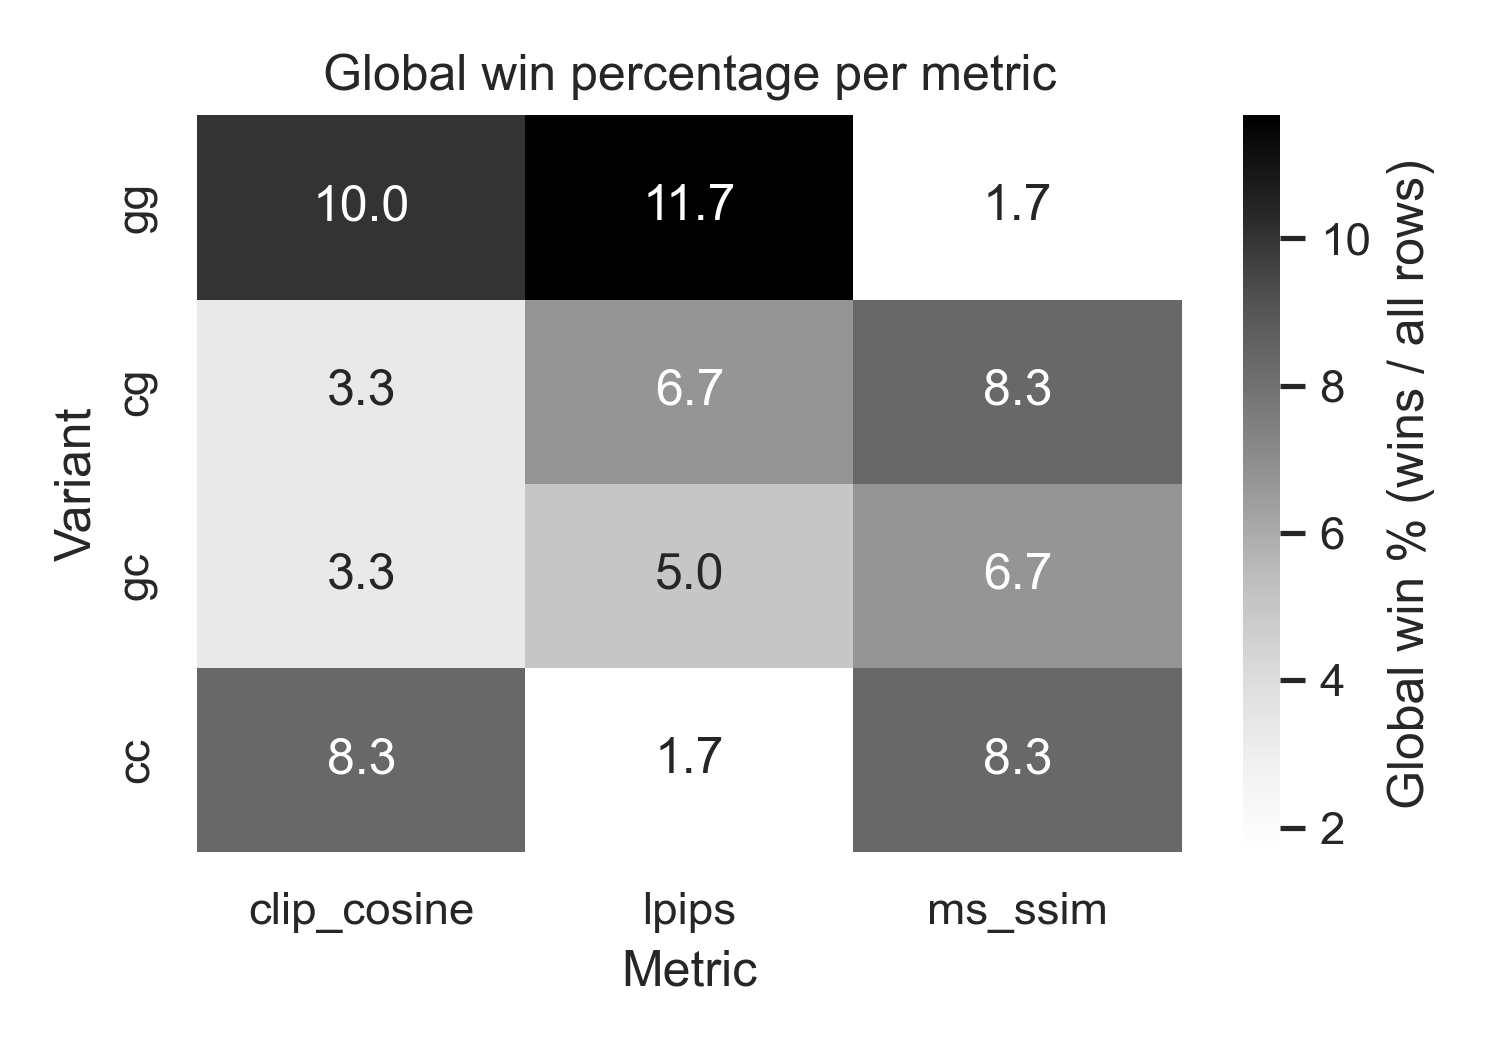
\includegraphics[width=\textwidth]{../03_project/01_basic/analysis/automatic_measures_report/metric_winners_heatmap.png}
      \end{center}
      \vspace{-2mm}
      %\scriptsize Per-image metric winners across variants.
    \end{column}
  \end{columns}
\end{frame}

% ----------------------------------------------------------
\begin{frame}{Metric Outcomes (RQ2) – Humans vs Metrics}
  \begin{columns}[T]
    \begin{column}{0.52\textwidth}
      \small
      \begin{itemize}
        \item Compare human top-1 frequencies with metric “winners”.
        \item Humans:
          \begin{itemize}
            \item Strong polarization toward (a).
          \end{itemize}
        \item Metrics:
          \begin{itemize}
            \item Spread wins across variants,
            \item Often pick different variants than humans.
          \end{itemize}
        \item \textbf{Takeaway:} No metric consistently selects the
              human favourite in this 4-way task.
      \end{itemize}
    \end{column}
    \begin{column}{0.45\textwidth}
      \begin{center}
        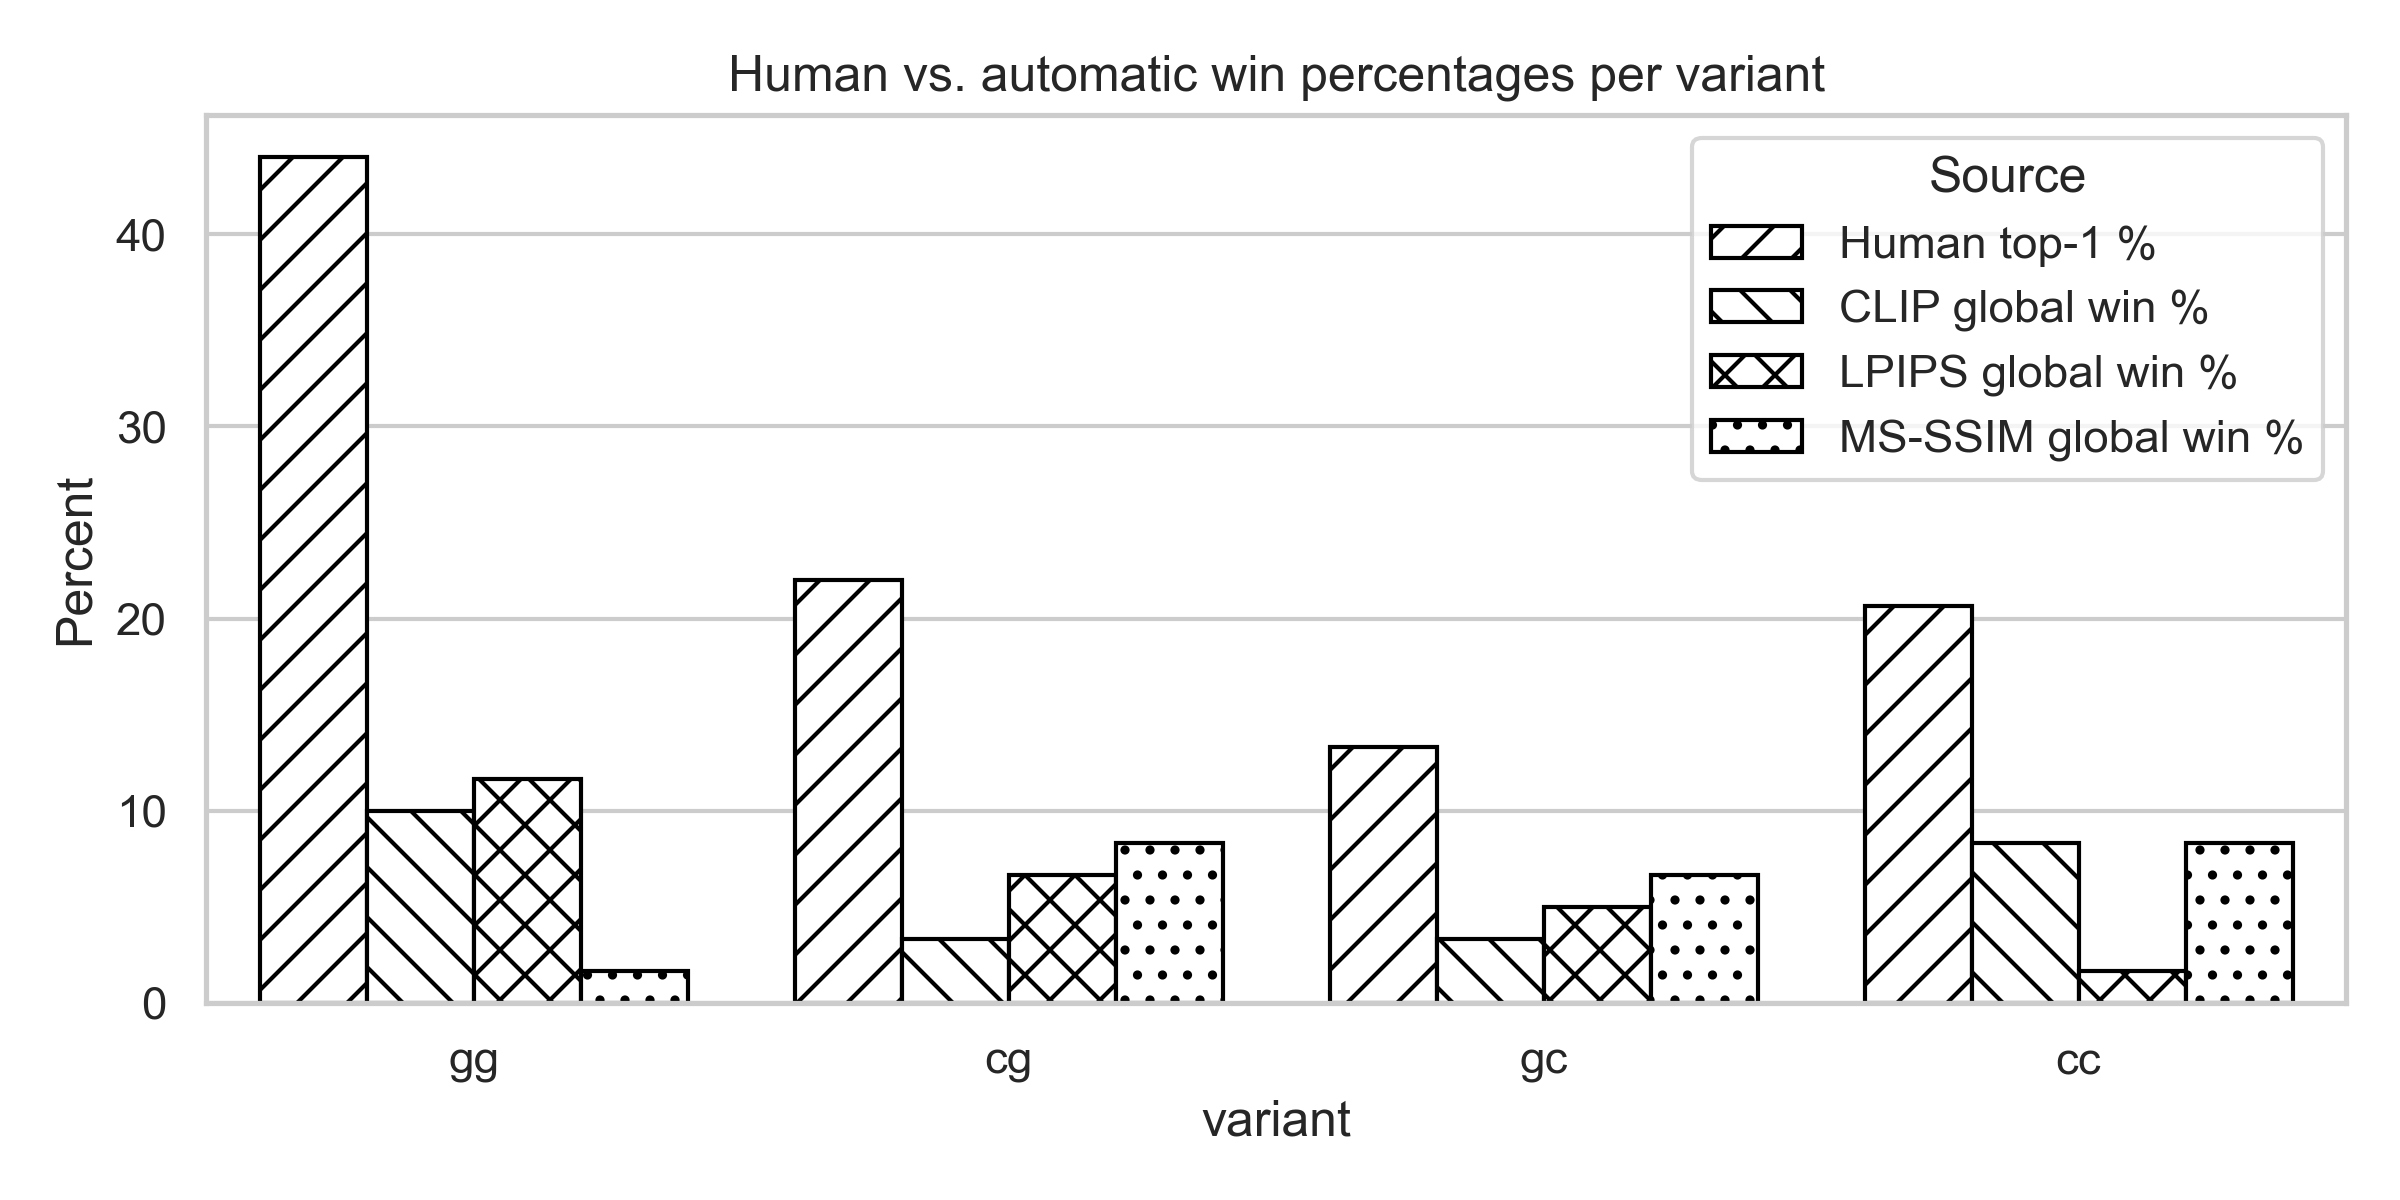
\includegraphics[width=\textwidth]{../03_project/01_basic/analysis/automatic_measures_report/human_vs_automatic_variants.png}
      \end{center}
      \vspace{-2mm}
      %\scriptsize Human vs metric top-1 rates across variants.
    \end{column}
  \end{columns}
\end{frame}

% ----------------------------------------------------------
\begin{frame}{Correlation Analysis (RQ2) – Mean correlations}
  \small
  \begin{itemize}
    \item Per image, I compute the correlation between
          \textbf{human mean ranks} and \textbf{metric-induced ranks}.
    \item Focus on Spearman (rank correlation), but Kendall and
          Pearson are also reported in the paper.
    \item Mean Spearman over 15 images:
      \begin{itemize}
        \item CLIP: \textbf{0.36}
        \item LPIPS: 0.11
        \item MS-SSIM: 0.06
      \end{itemize}
    \item \textbf{Interpretation}:
      \begin{itemize}
        \item CLIP tracks human rankings better on average.
        \item LPIPS and MS-SSIM show very weak average alignment.
        \item Still, even CLIP’s mean is far from a “strong”
              correlation.
      \end{itemize}
  \end{itemize}
\end{frame}

% ----------------------------------------------------------
\begin{frame}{Correlation Analysis (RQ2) – Uncertainty and tests}
  \begin{columns}[T,totalwidth=\textwidth]
    \begin{column}{0.52\textwidth}
      \footnotesize
      \begin{itemize}
        \item 95\% bootstrap CIs for mean Spearman (see plot):
          \begin{itemize}
            \item CLIP: 0.36 [\(-0.02\), 0.67]
            \item LPIPS: 0.11 [\(-0.25\), 0.46]
            \item MS-SSIM: 0.06 [\(-0.29\), 0.40]
          \end{itemize}
        \item All intervals include 0; CLIP’s band is shifted upward
              relative to the others.
        \item One-sided Wilcoxon tests on per-image Spearman:
          \begin{itemize}
            \item CLIP\textgreater LPIPS: \(p = 0.13\)
            \item CLIP\textgreater MS-SSIM: \(p = 0.07\)
          \end{itemize}
        \item \textbf{Takeaway:} CLIP is the least misaligned metric
              here, but its alignment is modest and not statistically
              significant; LPIPS and MS-SSIM are compatible with almost
              no correlation to human rankings.
      \end{itemize}
    \end{column}
    \begin{column}{0.45\textwidth}
      \begin{center}
        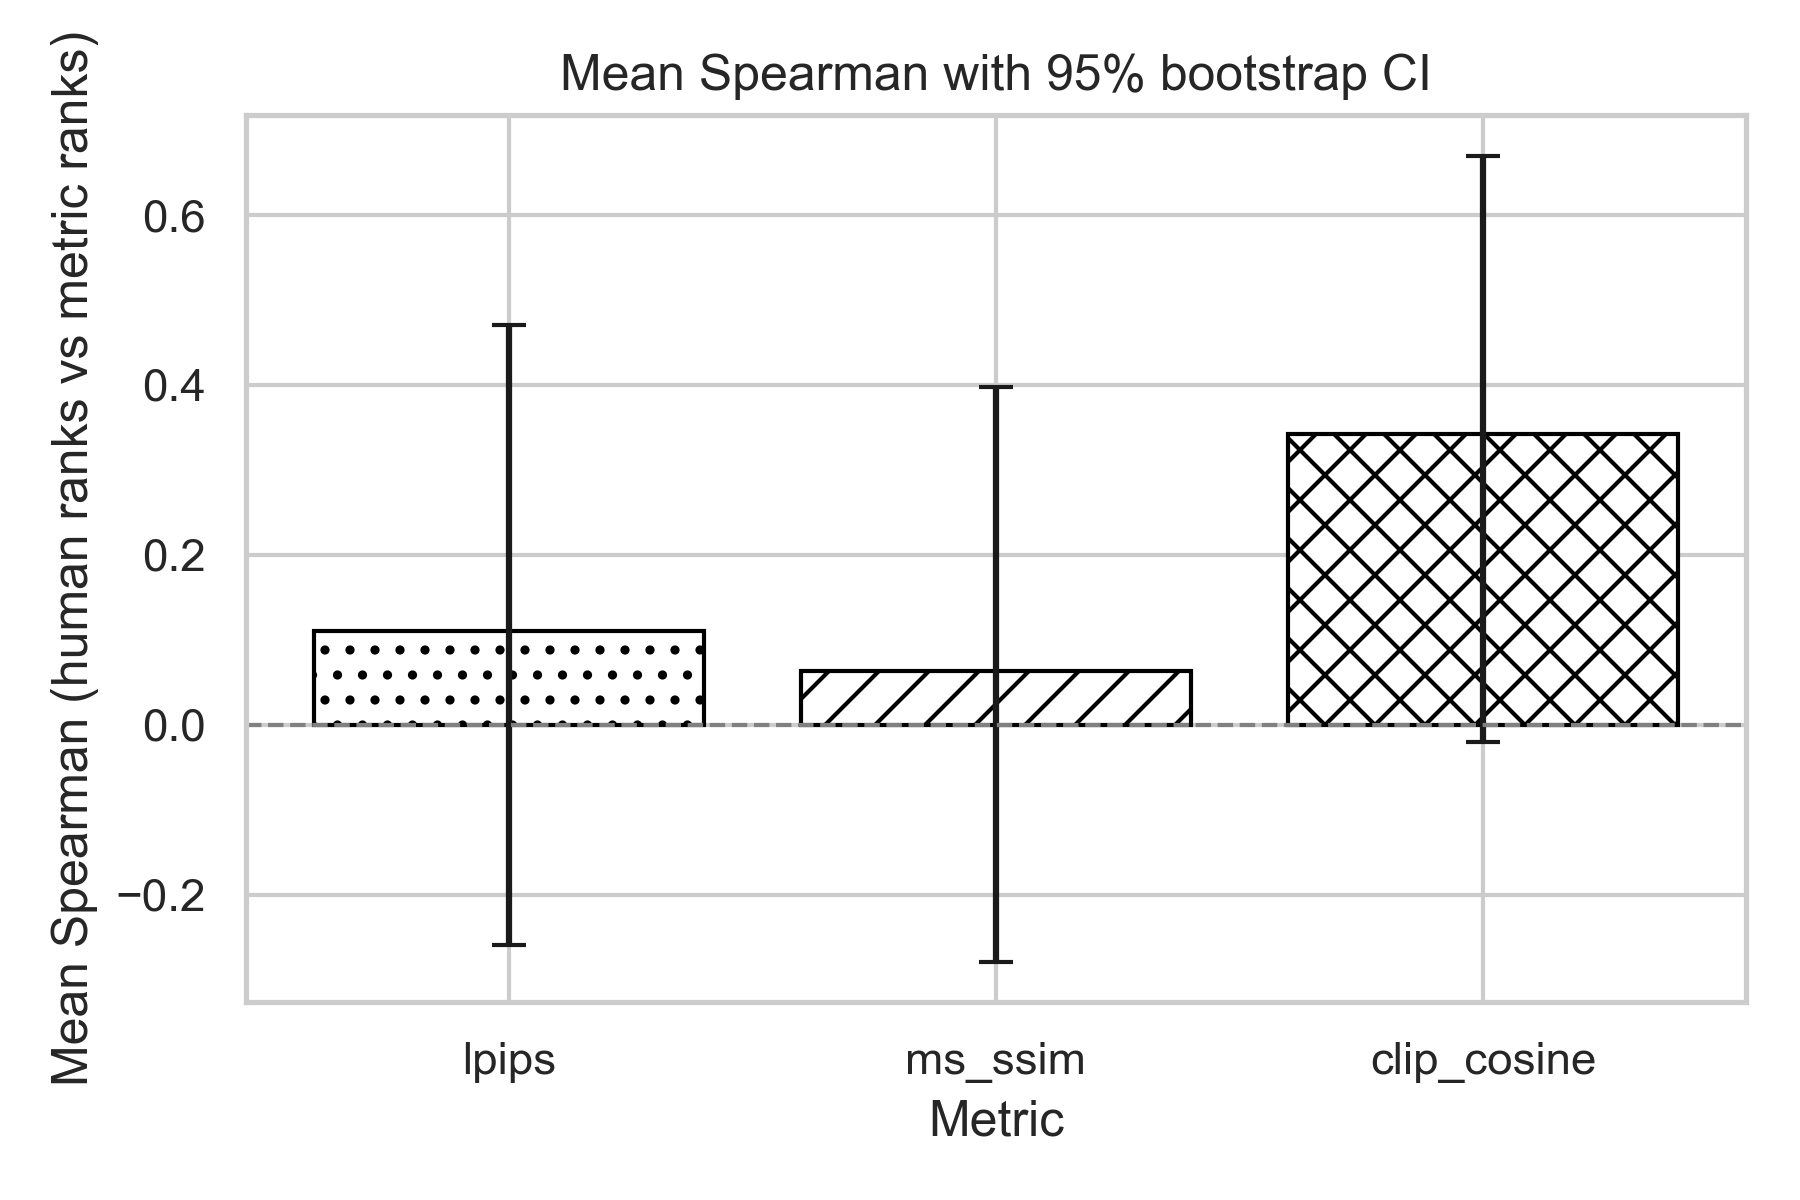
\includegraphics[width=\textwidth]{../03_project/01_basic/analysis/correlation_report/spearman_mean_ci.png}
      \end{center}
      \vspace{-2mm}
      %\scriptsize Mean Spearman correlation with 95\% bootstrap CIs.
    \end{column}
  \end{columns}
\end{frame}

% ----------------------------------------------------------
\section{Conclusions and Future Work}

\begin{frame}{Conclusions (RQ1)}
  \begin{itemize}
    \item Human raters show moderate agreement (\( \bar{W} = 0.40 \)).
    \item They clearly prefer Gemini-generated images with Gemini captions
          (variant (a)) in this setup.
    \item Intra-model consistency:
      \begin{itemize}
        \item Gemini with its own captions (a) vs Gemini with ChatGPT
              captions (b): strong preference for (a).
        \item ChatGPT with its own captions (d) vs Gemini captions (c):
              much smaller difference.
      \end{itemize}
    \item \textbf{Conclusion RQ1:} Gemini shows a higher intra-model consistency and a lower inter-model consistency than ChatGPT in this setting. ChatGPT shows a balanced inter- and intra-model consistency.
  \end{itemize}
\end{frame}

% ----------------------------------------------------------
\begin{frame}{Conclusions (RQ2) and Takeaways}
  \begin{itemize}
    \item CLIP shows the strongest (but modest) alignment with human
          rankings; LPIPS and MS-SSIM correlate weakly.
    \item No single off-the-shelf metric adequately proxies human
          judgments in this 4-way selection task.
    \item \textbf{Practical implications:}
      \begin{itemize}
        \item If forced to choose one metric, CLIP is a safer default
              than the other two here.
        \item Better: combine metrics and keep humans in the loop
              (e.g., human final selection from a shortlist).
      \end{itemize}
    \item Code, anonymized images, captions, and rankings:
          \texttt{https://github.com/SaverioNapolitano/qrd}
  \end{itemize}
\end{frame}

% ----------------------------------------------------------

\begin{frame}{Future Work}
  \begin{itemize}
    \item Larger studies with more images and raters.
    \item Explore other metrics (e.g., newer CLIP variants).
    \item Richer prompts.
  \end{itemize}
\end{frame}

\begin{frame}{Thank You}
  \begin{center}
    \LARGE Questions?
  \end{center}
\end{frame}

\end{document}
